% 2011 年重庆卷文科第 21 题：椭圆、准线 x=2√2 与点 P、M、N。
% 来源 PDF：普通高考/2011/2011重庆文.pdf，SHA-256 0ddbe738e4414213612fb6f62ec0c5cd252d039abf560bae1f31610558f93a70。
% 原页：第 2 页第 3 栏中部，书页码 654。示意。
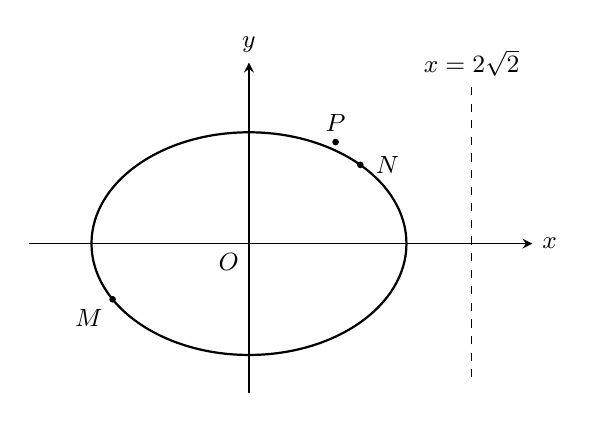
\begin{tikzpicture}[>=stealth, semithick, font=\small, scale=1.0]
  \draw[->] (-2.8,0)--(3.6,0) node[right] {$x$};
  \draw[->] (0,-1.9)--(0,2.3) node[above] {$y$};
  \draw[thick] (0,0) ellipse (2 and 1.414);
  \draw[dashed] (2.828,-1.7)--(2.828,2.0) node[above] {$x=2\sqrt2$};
  \fill (-1.732,-0.707) circle (1.2pt) node[below left] {$M$};
  \fill (1.414,1.0) circle (1.2pt) node[right=2pt] {$N$};
  \fill (1.10,1.29) circle (1.2pt) node[above] {$P$};
  \node[below left] at (0,0) {$O$};
\end{tikzpicture}
